\chapter*{Proposition 45}



\begin{figure*}[ht]
    \begin{center}
    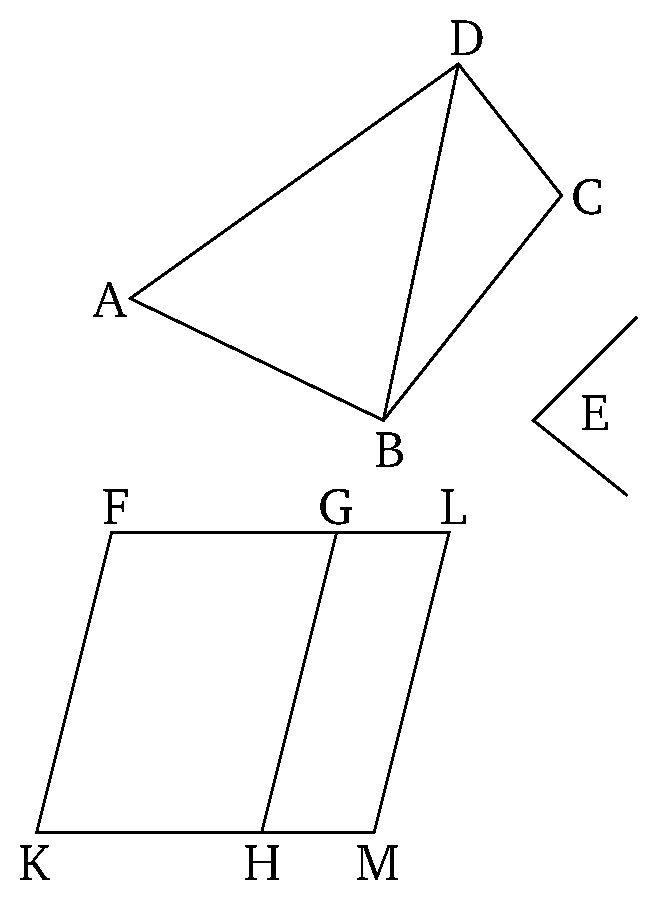
\includegraphics[width=0.5\linewidth]{figures/fig45e.eps}
    \label{fig:prop_45}
    \end{center}
\end{figure*}

To construct a parallelogram equal to a given rectilinear figure in a given
rectilinear angle.

Let $ABCD$ be the given rectilinear figure,$^\dag$ and $E$ the given rectilinear angle.
So it is required to construct a parallelogram equal to the rectilinear figure
$ABCD$ in the given angle $E$.

Let $DB$ have been joined, and let the parallelogram $FH$, equal to
the triangle $ABD$, have been
constructed in the angle $HKF$, which is equal to $E$ [Prop.~1.42].
And let the parallelogram $GM$, equal to the triangle $DBC$, have been
applied to the straight-line $GH$ in the angle $GHM$,
which is equal to $E$ [Prop.~1.44]. And since angle $E$ is equal to each of
(angles) $HKF$ and $GHM$,  (angle) $HKF$ is thus also equal to $GHM$. 
Let $KHG$ have been added to both. Thus, (the sum of) $FKH$ and $KHG$ is
equal to (the sum of) $KHG$ and $GHM$. But, (the sum of) $FKH$ and $KHG$ is equal to
two right-angles [Prop.~1.29]. Thus, (the sum of) $KHG$ and $GHM$ is also equal to
two right-angles. So two straight-lines, $KH$ and $HM$, not lying on the same side, make  adjacent angles with some straight-line $GH$, 
at the point $H$ on it, (whose sum is) equal to two right-angles.
Thus, $KH$ is straight-on to $HM$ [Prop.~1.14].
And since the straight-line $HG$ falls across the parallels $KM$ and $FG$, the alternate angles
$MHG$ and $HGF$ are equal to one another [Prop.~1.29]. Let $HGL$ have
been added to both. Thus, (the sum of) $MHG$ and $HGL$ is equal to 
(the sum of) $HGF$ and $HGL$.
But, (the sum of) $MHG$ and $HGL$ is equal to two right-angles [Prop.~1.29].
Thus, (the sum of) $HGF$ and $HGL$ is also equal to two right-angles.
Thus, $FG$ is straight-on to $GL$ [Prop.~1.14]. And since $FK$ is
equal and parallel to $HG$ [Prop.~1.34], but also $HG$ to $ML$ [Prop.~1.34],
$KF$ is thus also equal and parallel to $ML$ [Prop.~1.30]. And the straight-lines $KM$ and
$FL$ join them. Thus, $KM$ and $FL$ are equal and parallel as well [Prop.~1.33].
Thus, $KFLM$ is a parallelogram. And since triangle $ABD$ is equal to parallelogram $FH$, and $DBC$ to $GM$, the whole rectilinear figure
$ABCD$ is thus equal to the whole parallelogram $KFLM$.

Thus, the parallelogram $KFLM$, equal to the given
rectilinear figure $ABCD$, has been constructed in the angle
$FKM$, which is equal to the given (angle) $E$. (Which is) the very thing it was
required to do.


\section*{Commentary}

\begin{proposition}\label{proposition_45}\lean{Elements.Book1.proposition_45}\leanok
    If
\end{proposition}
\begin{proof}
    \uses{proposition_14,proposition_29,proposition_30,proposition_33,proposition_34,proposition_42,proposition_44}\leanok
\end{proof}
